% vim:ts=4:sw=4
% Copyright (c) 2014 Casper Ti. Vector
% Public domain.

\chapter{延迟环路PUF设计}\label{chap:dbrpuf}
在本章我们针对 BRPUF 进行改进,使 CRP 的统计分布趋于理想值。

\section{电路结构}\label{sec:dbrpuf_scheme}
从第\ref{chap:buildingmodel}章的讨论看出, BRPUF 输出分布扩散在(0,1)几乎呈均匀分布,这是 PUF 设计所不愿意看到的,其根本原因在于环路结构使得每一个环路中与非门的延迟波动产生叠加,造成了最终输出均值较大波动,在工艺方差不变的前提下,输出分布方差退化为工艺方差的N倍(N为级数),故N级数越高, BRPUF 输出分布越差。

结合 BRPUF 环路结构和仲裁 PUF 的延迟路径选择结构,提出了如图\ref{fig:dbrpuf}所示的电路,称为``延迟环路PUF''( Delay-based Bistable Ring PUF, DBRPUF )。

\begin{figure}[htb]
\centering
\includegraphics[width=\linewidth]{dbrpuf}
\caption{延迟环路PUF电路示意图}
\label{fig:dbrpuf}
\end{figure}

图\ref{fig:dbrpuf}所示结构由 $ N=2 $ 个单元构成,每个单元包含2个与非门和 $ K=4 $ 个双口交换器,其中交换器0--2由激励 $ c_0\sim c_2 $ 控制,最后一级交换器由 $ z_0=c_0\oplus c_1\oplus c_2  $ 控制使得最后一级交换器的底输出端口一定与顶与非门I0联接,而顶输出一定与底与非门I1相联接,因此每个单元有 $ k-1 $ 位激励输入,1位信号输入,1位信号输出和1位复位信号。N个单元输入输出连接成环路,在此结构中,由 $ 2N $ 个与非门组成了双稳态环路,激励信号 $ c_i $ 控制每个与非门的延迟路径,根据\ref{sec:brpufmodel}节理论,双稳环路的稳定态与环路中每一个与非门延迟相关,图\ref{fig:dbrpuf}中延迟可以看成与非门本征延迟和交换器延迟的累积,因此改变交换器状态即改变了环路中与非门的输入信号延迟时间,进而导致电路进入不同的稳态。故该PUF结构的CRP共有 $ 2^{N(K-1)} $ 对。

\section{统计分析}\label{sec:dbrpuf_stat}
设第i个单元中顶与非门I0和底与非门I1的总延迟分别为 $ (Sr_i^T,Sf_i^T),(Sr_i^B,Sf_i^B) $,其中 $ Sr $ 代表总上升沿延迟, $ Sf $ 代表总下降沿延迟。令信号从顶与非门I0输出的时刻为 $ p_0 $ ,底与非门I1输出的时刻为 $ q_0 $。每一级交换器j有4条路径,每条路径有上升延迟和下降延迟两个变量,用 $ (x_0^j,x_1^j,x_2^j,x_3^j) $ 表示4条路径的上升沿延迟,同理用 $ (y_0^j,y_1^j,y_2^j,y_3^j) $ 表示下降沿延迟。

首先考虑上跳沿的传输。

\begin{eqnarray}
p_{j+1}=\frac{1-c_j}{2}(p_j+x_0^j)+\frac{1+c_j}{2}(q_j+x_2^j) \\
q_{j+1}=\frac{1-c_j}{2}(q_j+x_3^j)+\frac{1+c_j}{2}(p_j+x_1^j)
\end{eqnarray}

两式相减得到类似仲裁型PUF延时差的表达式

\begin{equation}
\Delta_{j+1}=p_{j+1}-q_{j+1}=-\Delta_jc_j+\alpha_jc_j+\beta_j
\end{equation}

两式相加得到:

\begin{equation}
S_{j+1}=p_{j+1}+q_{j+1}=S_j+\gamma_jc_j+\tau_j
\end{equation}

其中 $ \alpha_j=\frac{x_0^j-x_1^j-x_2^j+x_3^j}{2},\beta_j=\frac{x_0^j-x_1^j+x_2^j+x_3^j}{2},\gamma_j=\frac{x_0^j-x_1^j-x_2^j+x_3^j}{2},\tau_j=\frac{x_0^j+x_1^j+x_2^j+x_3^j}{2} $。

递推可以得到 $ \Delta_K, S_K $ 的表达式。而
\begin{eqnarray}
p_K=\frac{S_K-\Delta_K}{2} \\
q_K=\frac{S_K+\Delta_K}{2}
\end{eqnarray}

故I0传递到I1信号上升沿延迟 $ Sr_i^T=q_K-p_0 $,I1传递到输出端口的上升沿延迟 $ Sr_i^B=p_K-q_0 $。

同理可得,下降沿延迟具有相同的表达式,只是式中变量含义不同。

根据双稳态环路的稳定判据,可推出:

\begin{equation}\label{eq:dbrpufmodel}
R=sgn[\sum\limits_{i=0}^{N}[(Sr_i^T-Sf_i^T)-(Sr_i^B-Sf_i^B)]]=sgn[\sum\limits_{i}^{N}(\Delta r_K-\Delta f_K+\Delta_0)]
\end{equation}

其中 $ \Delta r $ 具体指上升沿延迟差,$ \Delta f $ 指下降沿延迟差,$ \Delta_0 $ 是常数偏置,其物理意义是信号进入交换器的时刻差 $ p_0-q_0 $,我们希望没有偏置,即$ \Delta_0=0 $,而则可以通过合理布局布线达到。由于$ \Delta r $和$ \Delta f $具有相同的表达形式$ \Delta=P'D $,式\ref{eq:dbrpufmodel}可以变为:

\begin{equation}
R=sgn[\sum\limits_{i}^{N}P'_i(D_i^1-D_i^2)]=sgn[\sum\limits_{i}^{N}P'_iD_i]
\end{equation}

最终简化成了N个子单元中延迟差的和。与仲裁型 PUF 具有相似的形式。

令$ \delta=\sum P'D $,由\ref{subsec:brpuf_stat}节相关推论可知,$ \delta $的均值分布的方差由 BRPUF 的 $ N=32 $ 倍于单元延迟方差,缩小到 $ N=4 $ 倍,而 CRP 则由 $ N\times (K-1)=32 $ 保持与 BRPUF 一致。

\section{仿真验证}
采用 SMIC 40nm 工艺制程,用 HSPICE 库进行蒙特卡洛仿真提取延迟参数,再带入 Matlab 脚本生成模拟电路矩阵,得到$ 1000\times 1000 $的 CRP 矩阵。
表[]列出了电路参数;图\ref{fig:dbrpuf_dist}展示了改进的 DBRPUF 的随机性分布和独特性分布图。

\begin{figure}[htb!]
\centering
\subfloat[随机性]{
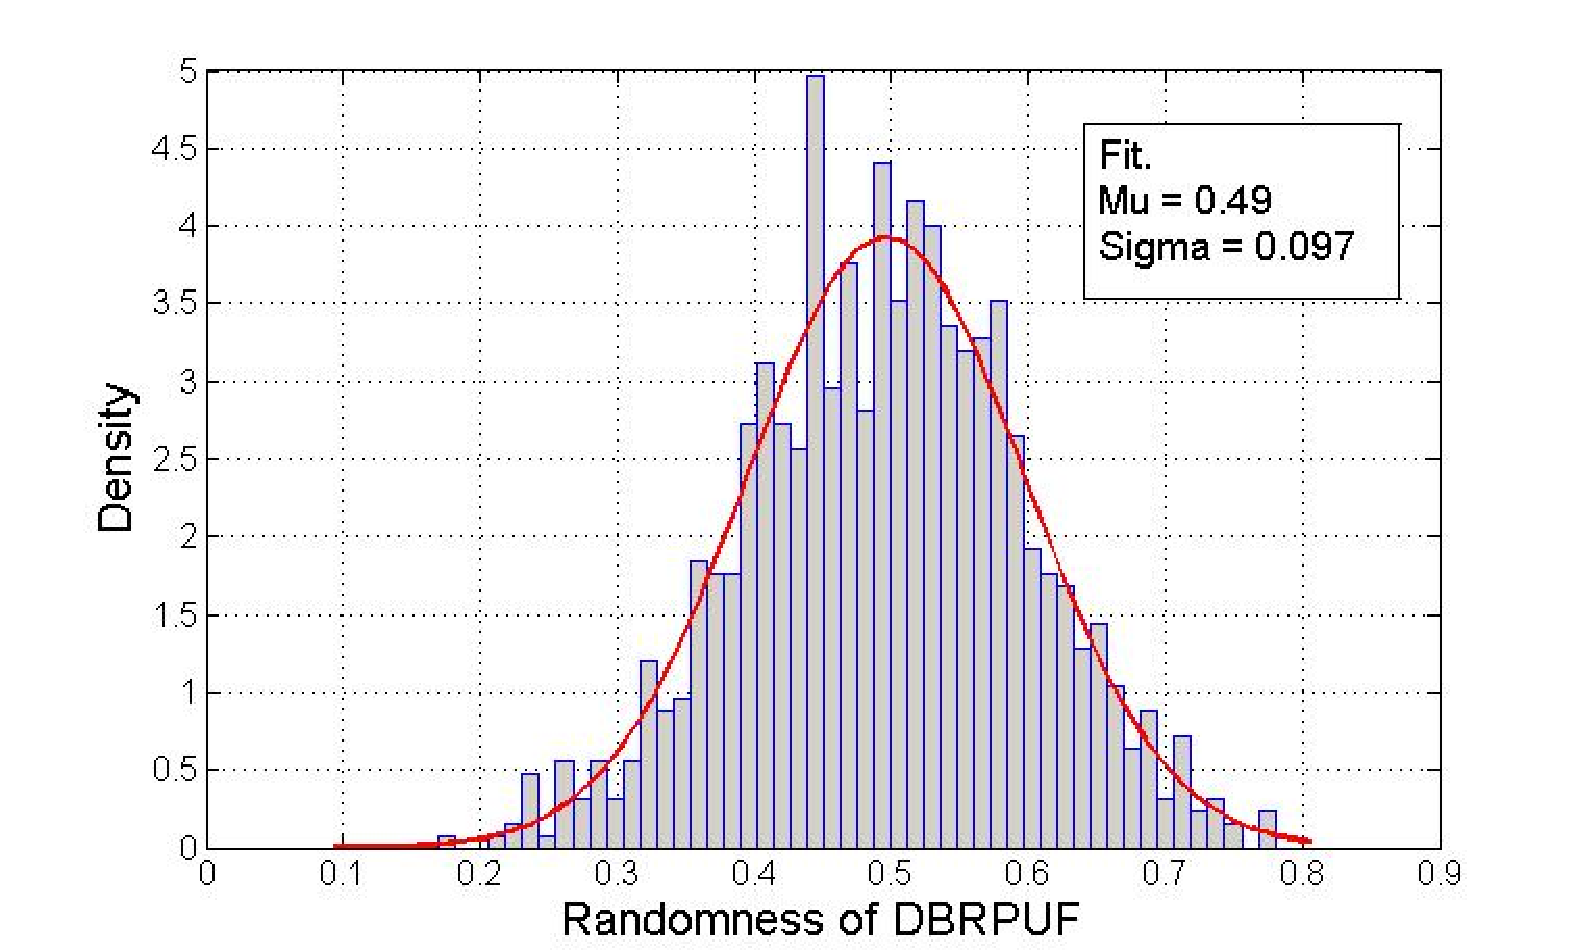
\includegraphics[width=.5\linewidth]{dbrpuf_rand_simulation}
}
\subfloat[独特性]{
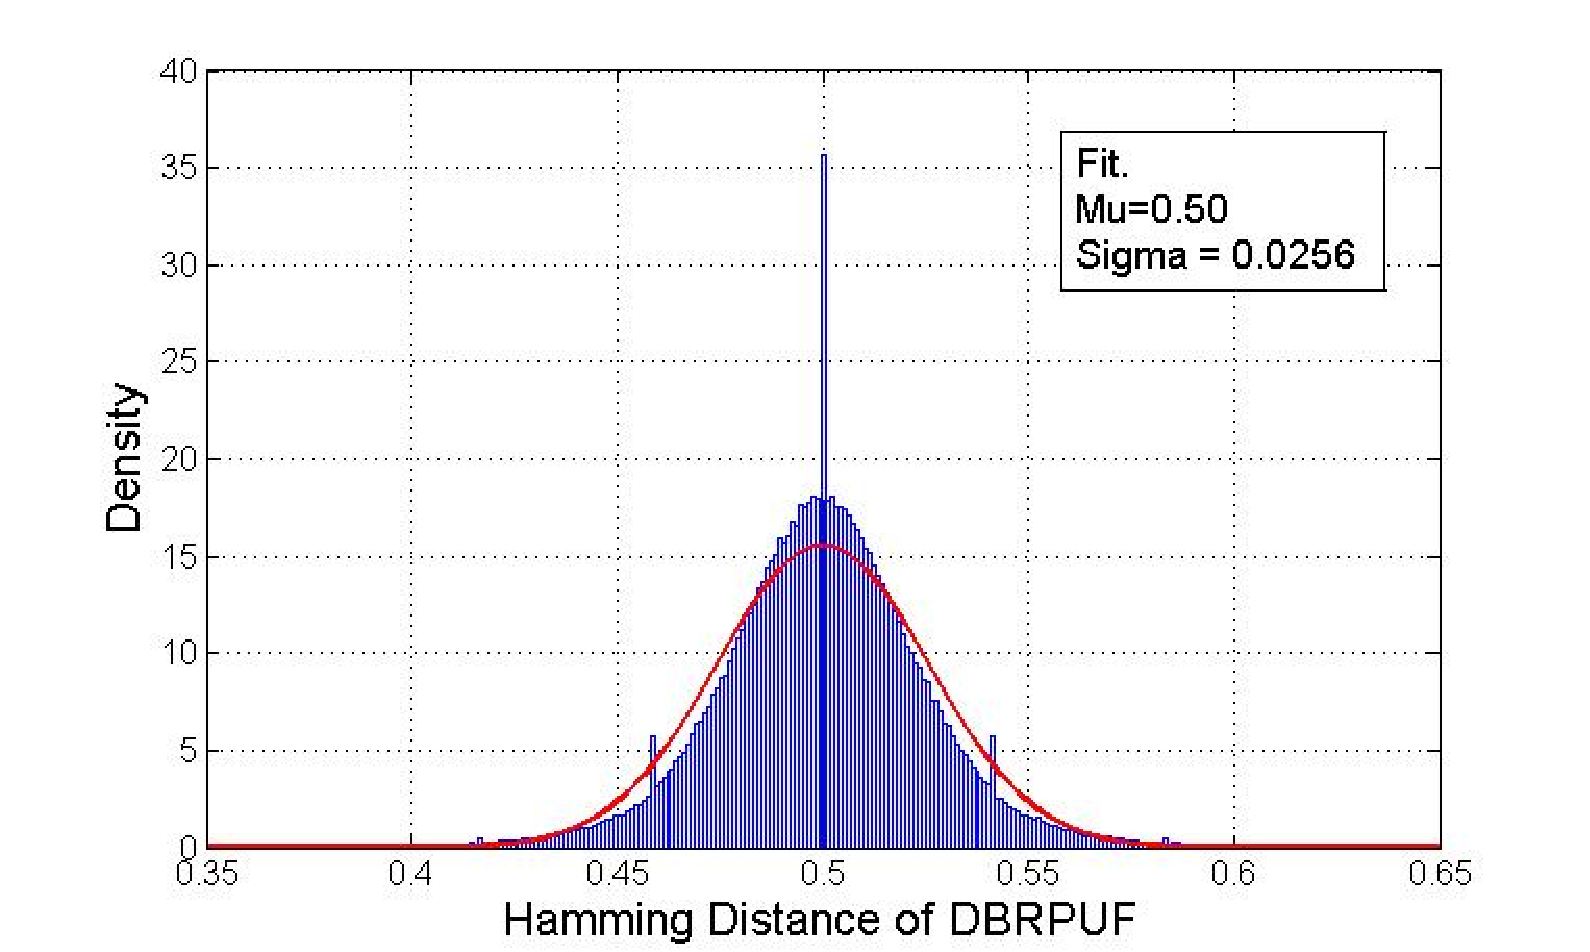
\includegraphics[width=.5\linewidth]{dbrpuf_uniq_simulation}
}
\caption{DBRPUF分布图}
\label{fig:dbrpuf_dist}
\end{figure}

可以看出 DBRPUF 的随机性分布达到 $ N_rand\sim(0.49,0.097) $,独特性分布达到 $ N_uniq\sim(0.50,0.0256) $,满足上小节的理论分析。相比于 BRPUF 大大改善了输出分布情况。但是 DBRPUF 的 CRP 仍然是n维空间线性可分,其复杂度与传统仲裁型 PUF 和 BRPUF 相当,为了提高模型复杂度必须采用多 PUF 单元异或的方式,无疑增加了电路的面积功耗开销,不利于 PUF 的实现。


\section{FPGA实现}
采用 Altera Stratix V 芯片,用3块 FPGA 综合并实现 DBRPUF 设计。图 17展示了 DBRPUF 实现的 Chip plan,我们用一个 LUT 实现交换器,故每一个单元级需要$ K+2 $个 LUT 实现$ K $个交换器和2个与非门。与 BRPUF 一样,需要手动设计 LUT 的摆放位置以保证布线的平衡。读出逻辑采用 250 MHz 时钟连续采样,若在 1000 个时钟周期内存在100个连续稳定的值则视其为输出,保存在输出寄存器中。寄存器的值和控制逻辑通过 PCI-E 接口与 PC 相连。

\begin{figure}[htb]
\centering
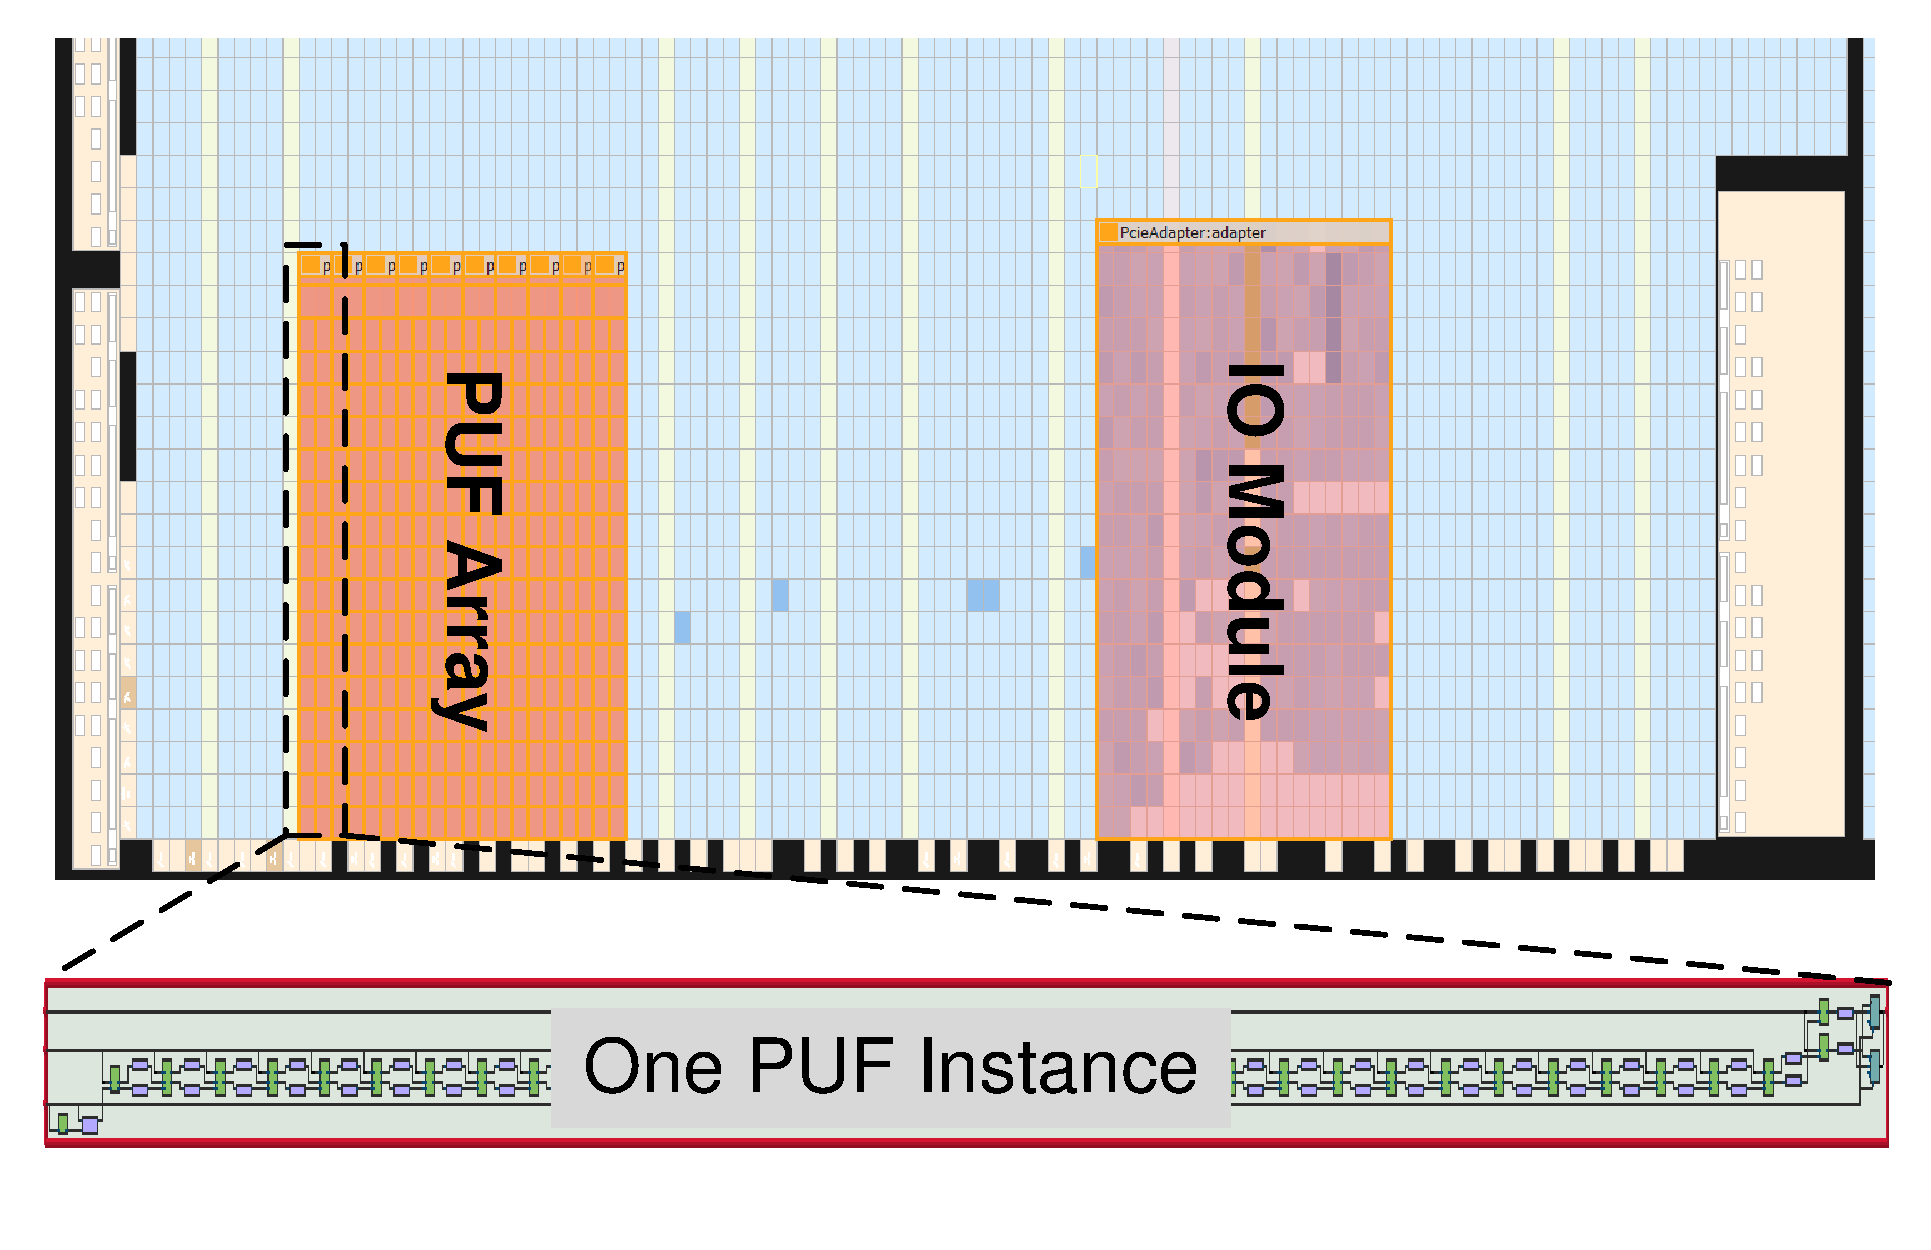
\includegraphics[width=.8\linewidth]{dbrpuf_cp}
\caption{DBRPUF在FPGA的Chipplan示意图}
\label{fig:dbrpuf_chipplan}
\end{figure}

在每块 FPGA 芯片的不同位置摆下10个 DBRPUF,共享一个读出逻辑,一共30个独立 PUF 元件。每个 PUF 等概率给予5000个随机32位激励,每个激励重复100次以验证可重复性,记录输出寄存器共 $ 30\times 5000\times 100 $ 个输出,经过 Matlab 统计分析,得到 DBRPUF 的随机性、独特性和可靠性分布。如图\ref{fig:dbrpuf_dist_fpga}所示, DBRPUF 的独特性满足 $ N\sim(0.494,0.0048) $ 的高斯分布,可靠性满足 $ N\sim(0.057,0.013) $ 的高斯分布(随机性样本太少不做统计)。

\begin{figure}[htb!]
\centering
\subfloat[FPGA随机性]{
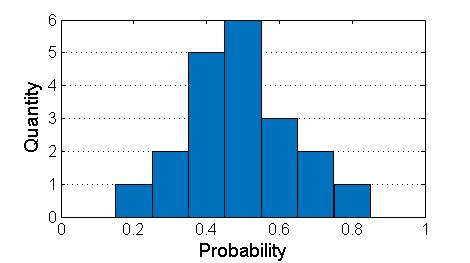
\includegraphics[width=.5\linewidth]{dbrpuf_rand_fpga}
}\\
\subfloat[FPGA独特性和可靠性]{
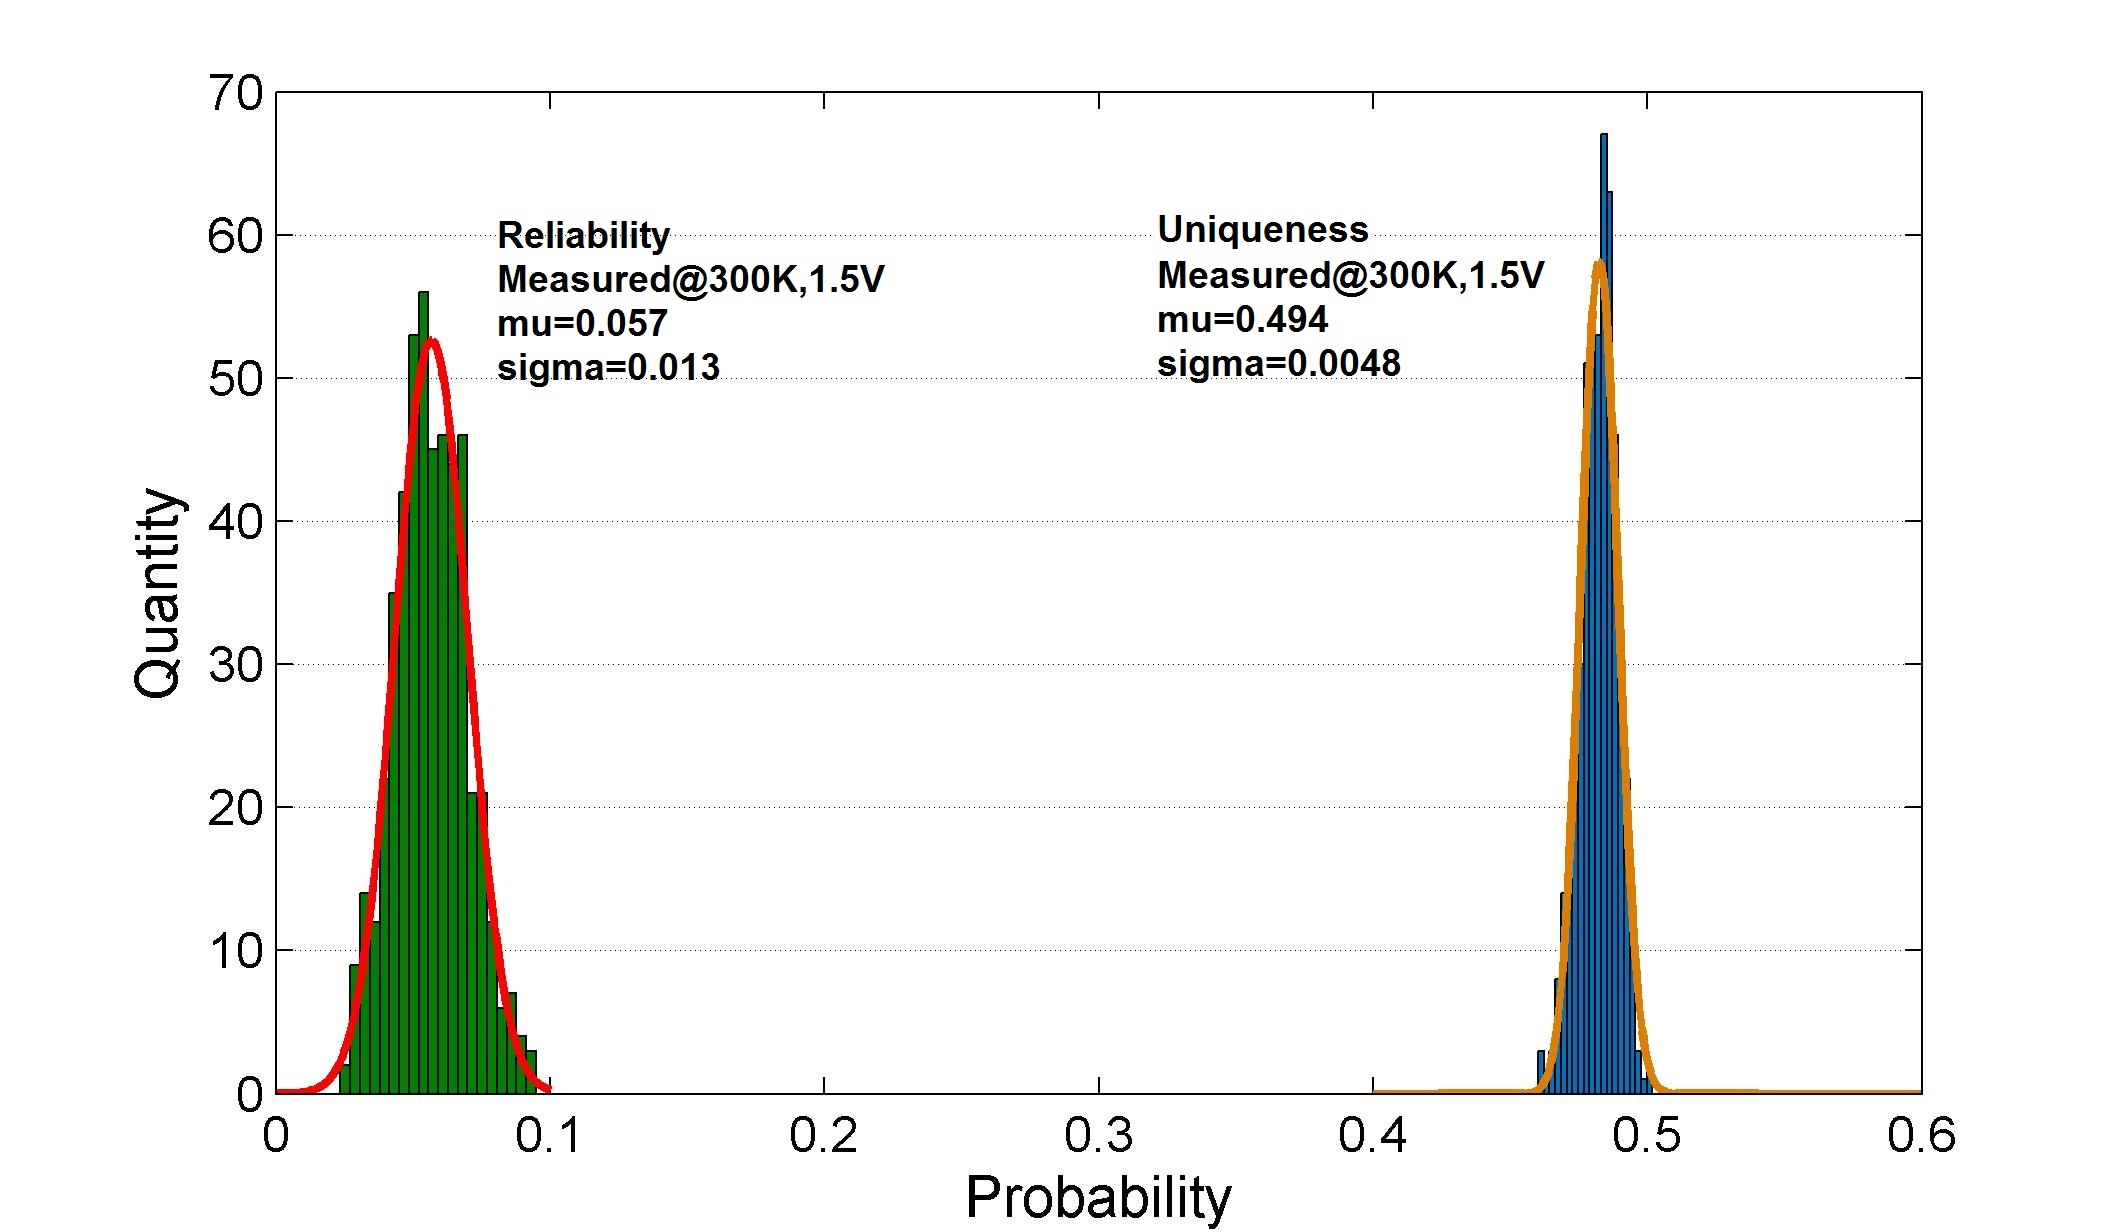
\includegraphics[width=.8\linewidth]{dbrpuf_uniq_fpga}
}
\caption{FPGA实现DBRPUF分布图}
\label{fig:dbrpuf_dist_fpga}
\end{figure}


\section{本章小结}
本章基于 BRPUF 和交换器设计了一种新型 PUF 结构,称为延迟双稳环路 PUF ( Delay-based Bistable Ring PUF )。
DBRPUF 改善了 BRPUF 分布分散的缺点,使得统计特性比 BRPUF 更好。并且从理论、仿真与 FPGA 三方面验证了这一结论。

但 DBRPUF 相比于传统仲裁型 PUF 并没有显著优势,其分布结果也没有达到最理想的效果,但是从 SVM 学习效果来看, DBRPUF 在一定程度上增加了学习复杂度,提高了求解时间代价。
